\chapter{Einleitung}

\section{Motivation}
Um im Unterricht Schülern und Studenten dass Programmieren und Konstruieren von Robotern zu erläutern, ist Lego Mindstorms mit dem programmierbaren Baustein NXT eine gute Wahl. Das Ziel dieser Arbeit ist es das programmieren von Lego Mindstorms Robotern zu vereinfachen und gleichzeitig die Grenzen die duch den Baustein NXT gesetzt sind zu sprengen. Wir wollen die Möglichkeiten der Programmierung des NXT eins zu eins mit dem Minicomputer Raspberry PI abbilden. Damit ist es uns möglich eine einfachere Programmierschnittstelle anzubieten und zusätzlich die vielen Möglichkeiten des Raspberry PIs für Schüler zugänglich machen. 

In der Folgenden Arbeit werden wir den, vom Raspberry PI gesteuerten, Lego Mindstorms Roboter LegoPI nennen.

Wir sehen den Raspberry PI als ein dem NXT überlegenes Steuerungsmodul, da auf dem Raspberry ein vollständiges Ubuntu Linux Betriebssystem läuft. Eine Überlegung der Autoren hierbei war es auf dem Ubuntu einen Webserver laufen zu lassen und dem Roboter über diesen aus der Ferne zu steuern.
Weiterhin soll es in dieser Arbeit ermöglicht werden, weitere Sensoren an den Raspberry PI anschließen zu können. Zwar gibt es für Lego Mindstorms eine Liste von Sensoren, wie z.B einen Lichtsensor, Tastsensor und Ultraschallsensor, dieses Set an Sensoren ist allerdings eingeschränkt.

Das Bereitstellen eines programmierbaren Roboters für jeden Schüler kann schnell teuer werden. Wir sehen die Verwendung eines Raspberry PI auch deshalb als Vorteil, weil ein Raspberry B+ mit 39,90 Eur den NXT mit 9841 mit 148,99 Eur preislich schlägt. \footnote{Preisvergleich des Raspberry PI 2 B+ und NXT 9841 auf www.amazon.de}

In dieser Arbeit werden wir uns darauf beschränken alle Sensoren des NXT Bausatzes mit dem Raspberry PI zu verbinden. Zusätzlich soll es möglich sein Motoren über den Raspberry zu steuern. Um zu Prüfen ob der Raspberry PI den NXT im Unterricht ersetzen kann, werden wir einen Parqour der auch von Schülern der Hochschule Mannheim absolviert werden muss mit dem LegoPI durchlaufen.

\chapter{Grundlagen}
\section{Raspberry PI}
\label{Grundlagen:RaspberryPI}
%\index{Auszeichnungen!im Text}

Raspberry PI ist ein günstiger Computer in Kreditkartengröße, welches viele Schnittstellen bietet, wie z.B HDMI, USB, Audio, GPIOs und Ethernet.
Was den Raspberry PI so beliebt macht um eigene Systeme zu bauen, ist dass auf ihm ein vollständiges Linux Betriebssystem läuft. Dies führt dazu, dass nahezu alles was auf einem Desktoprechner läuft auch auf einem Raspberry PI ausführbar ist.

\begin{figure}[h]
  \centering
  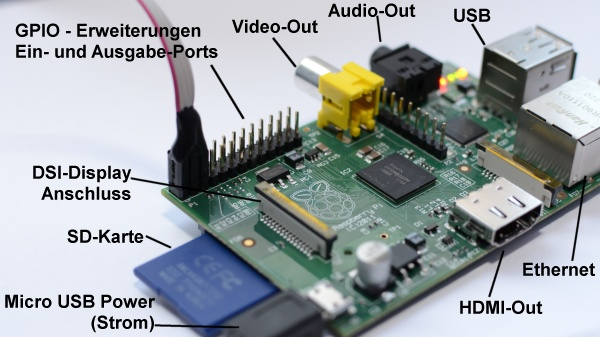
\includegraphics[width=15cm]{raspberrypi}
  \caption{Ein RaspberryPI 2 mit Beschrifteten Schnittstellen. Quelle: http://www.portunity.de/blog/2013/februar/raspberry-pi-warum-ist-der-mini-computer-bei-unseren-mitarbeitern-so-beliebt.html}
  \label{Kap1:RaspberryPI}
\end{figure}

\section{NXT}
\label{Grundlagen:NXT}
%\index{Auszeichnungen!im Text}

Lego Mindstorms NXT ist ein Steuerungscomputer der Produktserie Lego Mindstorms. Es hat ebenso wie der Raspberry PI Anschlüsse für USB- und Bluetooth Schnittstellen. Im Gegensatz zu Raspberry PI bietet der NXT schon von vornerein Anschlüsse für Sensoren und Aktoren. 

\begin{figure}[h]
  \centering
  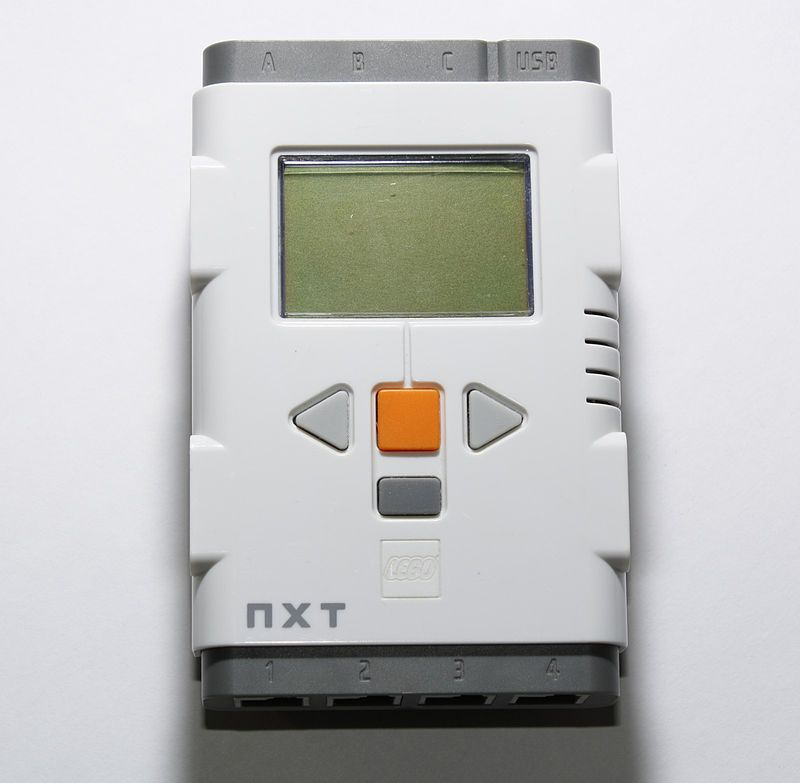
\includegraphics[width=12cm]{nxt}
  \caption{Ein NXT Baustein mit Anschlüssen für Motoren und Sensoren. Quelle: https://de.wikipedia.org/wiki/Lego-Mindstorms-NXT}
  \label{Kap1:NXT}
\end{figure}

\section{A/D-Wandler}

Ein Analog-Digital-Umsetzer, kurz A/D-Wandler, ist ein elektronisches Baustein, bei dem ein zeit-kontinierliches Eingangssignal in einzelne diskrete Abtastwerte abgetastet werden.

In folgender Abbildung ist ein MCP3008 abgebildet. In dieser Arbeit wird dieser Baustein dazu verwendet, analoge Signale von Lego Sensoren in digitale Daten abzutasten, um diese im Raspberry PI zu verarbeiten. Der MCP3008 bietet 8 Eingänge um Sensoren Anzuschließen.

\begin{figure}[h]
  \centering
  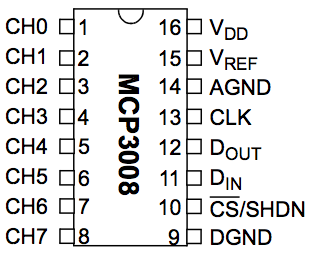
\includegraphics[width=12cm]{mcp3008}
  \caption{MCP3008 A/D-Wandler mit 8 Eingängen für Sensoren CH0-CH7}
  \label{Kap1:NXT}
\end{figure}

\section{Bussysteme}
In der Computerarchitekture ist ein Bus ein System, das Daten zwischen einzelnen Computerbestandteile überträgt.

\subsection{SPI}

Der Serial Peripheral Interface (SPI) Bus ist eine von Motorola entwickelte,  synchrone serielle Kommunikationsschnittstelle, welche für die Übertragung von Daten über kurze Distanzen entworfen ist.  Häufige Anwendung findet der SPI in Embedded Systems. 

Eine Kommunikation über SPI erfolgt über einen SPI Master und einen SPI Slave. Der SPI Master startet eine Kommunikation in dem er die SS Verbindung auf 0 Volt zieht und eine clock signal mit einer bestimmten clock frequency aktiviert. Die zu sendenden Signale werden dann über den MOSI (Master Out Slave In) übertragen, in der Frequenz die von SCLK vorgeben ist. Der SPI ist ein single-master Protokoll, da lediglich ein Master die Kommunikation über alle Slaves steuert.

\begin{figure}[h]
  \centering
  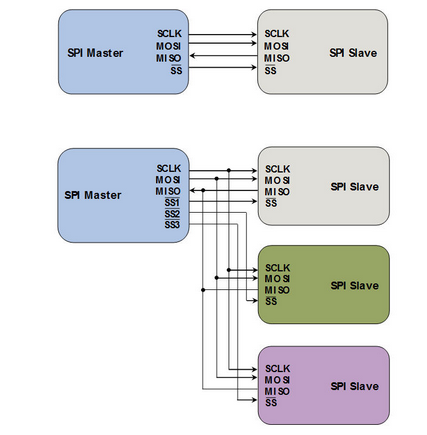
\includegraphics[width=12cm]{spi.png}
  \caption{SPI Kommunikation erfolgt über einen Puls der von SCLK gegeben ist und den Master und Slave synchronisiert. Über MOSI (Master IN Slave OUT) sendet der Master Signale an den Slave. Quelle: http://www.byteparadigm.com/applications/introduction-to-i2c-and-spi-protocols}
  \label{Kap1:SPI}
\end{figure}

\subsection{I2C}

I2C ist ein multi-master Protokoll mit zwei Datenleitungen. Über Serial Data (SDA) werden die Daten übertragen. Der SCL (Serial Clock) gibt die Frequenz der Datenübertragung an und synchronisiert somit die Kommunikationspartner. Jedes Gerät, welches an den Bus angeschlossen ist bekommt eine 7 -bit slave address. Es können beliebig viele Geräte an den I2C angeschlossen werden. Die Daten werden in 8-bit Paketen übertragen. Die Daten Raten können 100 kbps, 400 kbps oder 3.4 Mbps betragen. Diese verschiedenen Übertragungsraten werden auch standard mode, fast mode und high speed mode genannt.

Physikalisch besteht der I2C Bus aus zwei Leitungen und einer Ground Leitung (FIXME:siehe Abbildung x). Die aktiven Leitungen sind bi-direktional. Im I2C Standard ist definiert, dass jedes I2C Gerät welches Daten übersenden will, die Rolle eines Masters annimmt und alle anderen Geräte in diesem Moment Slaves sind.

\begin{figure}[h]
  \centering
  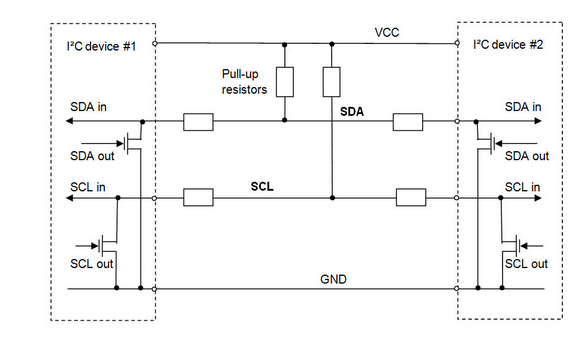
\includegraphics[width=15cm]{i2c}
  \caption{Zwei I2C Geräte sind über SDA und SCL verbunden. Diese beiden Leitungen sind über pull-up Widerständen mit VCC verbunden. Quelle: http://www.byteparadigm.com/applications/introduction-to-i2c-and-spi-protocols/}
  \label{Kap1:I2C}
\end{figure}

\subsection{Sensoren}
Unter Sensoren versteht man Komponenten, in denen eine physikalische oder chemische Veränderung in ein geeignetes Nutzsignal erfasst oder gemessen wird. \cite{FIXME: }

Im folgenden werden die Sensoren beschrieben, die in dieser Arbeit in Betrieb genommen werden.

\subsubsection{NXT Lightsensor}
Der NXT Lichtsensor misst wie viel Licht  in den Sensor fällt. Dies geschieht über einen light-dependent resistor (LDR), der ein variabler Widerstand ist der niedriger wird, je mehr Licht in hereinfällt. Der Lichtsensor verfügt ebenfalls über eine externe Lichtquelle. Mit dieser ist es möglich auch in dunklen Lichtverhältnissen zwischen Oberflächen zu unterscheiden.

\begin{figure}[h]
  \centering
  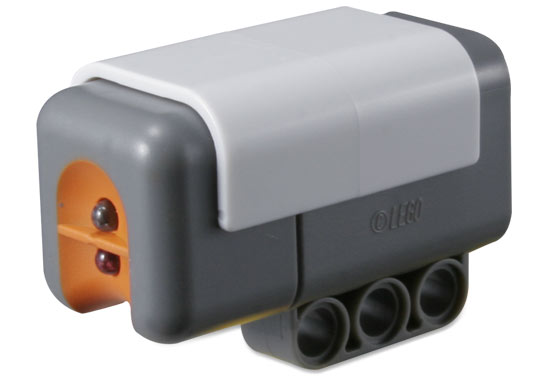
\includegraphics[width=6cm]{lightsensor}
  \caption{NXT Lightsensor mit dem LDR oben und einer externen Lichtquelle unten.}
  \label{Kap1:Lightsensor}
\end{figure}

\subsection{Tastsensor}

Der Tastsensor ist ein einfacher Sensor der die Werte 1 für gedrückt und 0 für nicht gedrückt darstellen kann. In dieser Arbeit wird dieser Sensor beispielsweise dazu verwendet den Roboter zu starten. Ist der Schalter gedrückt, wird ein Startskript ausgeführt.

\begin{figure}[h]
  \centering
  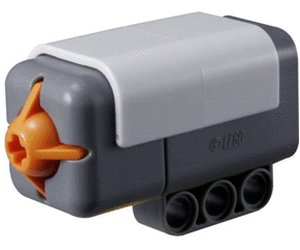
\includegraphics[width=6cm]{tast}
  \caption{NXT Tastsensor}
  \label{Kap1:tast}
\end{figure}

\section{PWM}

\section{GPIO}
Ein General Purpose Input/Output (GPIO) ist eine einfache digitale Schnittstelle mit der eine Folge von einsen und nullen übertragen werden können.
Der Raspberry PI 2 bietet 40 GPIOs, welche jeweils als Eingabe oder Ausgabe Pins geschaltet werden können.

\chapter{Implementierung}

\section{Herausforderungen beim Auslesen der Sensoren}

Den ersten Sensor den wir ausgelesen haben war der Tastsensor. Diesen haben wir über einen GPIO direkt mit dem Raspberry PI verbunden.
Über das öffnen des GPIOs via RPi.GPIO konnten wir auslesen, ob der Tastsensor gedrückt ist oder nicht. 

Die Idee war den Lichtsensor auch über GPIO auslesen zu können. Eine solche Testkonfiguration zeigte allerdings, dass wir keine sinnvollen Werte über den GPIO auslesen können. 

Eine weitere möglichkeit sahen wir darin, über I2C den Sensor anzuschließen. Leider zeigte auch diese Option keinen Erfolg, da die NXT Sensoren eine eigenes I2C  Protokoll verwenden, welches nicht kompatibel ist mit dem I2C Bus am Raspberry PI. 

Eine funktionierende Lösung sah so aus, den Sensor mit einem A/D-Wandler zu verbinden und dann per GPIO die digital abgetasteten Daten zu empfangen. Da wir keinen A/D-Wandler zur Verfügung hatten, bauten wir uns einen eigenen A/D-Wandler. (vgl. Abbildung xx FIXME). Der Nachteil dieser Schaltung ist, dass lediglich ein Sensor ausgelessen werden kann. Um den Anforderungen gerecht zu werden und einen Parqour wie in der Robotik Vorlesung zu durchlaufen ist der Einsatz von mehreren Sensoren notwendig. Dies erreichten wir mit dem Einsatz eines MCP3008 A/D-Wandler. Mit diesem ist das Auslesen von bis zu 8 Sensoren gleichzeitig möglich. (vergleiche xx FIXME).

\begin{figure}[h]
  \centering
  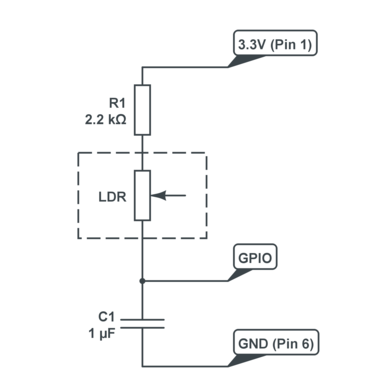
\includegraphics[width=10cm]{adwandlereigen}
  \caption{A/D-Wandler realisiert über einen LDR der in Reihe geschaltet ist mit einem 2.2 kOhm Widerstand und 1$\mu$F Kondensator}
  \label{Kap1:Lightsensor}
\end{figure}


\chapter{Fazit}

In dieser Arbeit haben wir es geschafft LegoPI zu bauen. Einen Roboter der mit allen analogen Sensoren des Lego Mindstorms Bausatzes kompatibel ist. LegoPI ist ebenso in der Lage zwei Motoren zu steuern, um die Fortbewegung des Roboters zu ermöglichen. Wir konnten einen einfachen Parqour durchlaufen, in welchem der Roboter einer schwarzen Linie folgt und am Ende an einer Wand stehen bleibt. Das Signal zum Stehenbleiben wird hier über einen Tastsensor ausgelöst, welcher an der vorderen Front des Roboters angebracht ist. FIXME: Bild?




\blindtext[4]